W tej sekcji zbadano jak dobrze model radzi sobie z różnymi obiektami należącymi do tej samej klasy. Umiejętność generalizacji zostanie sprawdzona na przykładzie klasy \emph{krzesło} (ang. \emph{chair}). Użyte obiekty to krzesło oraz fotel dla graczy (dalej zwany fotelem). Nazwy angielskie tych obiektów to kolejno \emph{chair} i \emph{gaming chair}, jest to ważne, ponieważ klasy COCO zostały stworzone według angielskiego nazwenictwa, na którego podstawie przypisuje się rózne warianty obiektów do jednej klas.  W badaniu tym porównano wyniki dla krzesła i fotela w funkcji progu ufności dla wszystkich (czterech) poziomów ośwetlenia. Do testu wykorzystano osiem filmów -- cztery z widocznym krzesłem i człowiekiem, cztery z widocznym fotelem i człowiekiem. Wartości jasności i nasycenia dla każdego filmu ukazono w tabeli \ref{tab:jasnosc-krzeslo-fotel}. Wygląd nagranego pomieszczenia wraz z nagranym obiektem dla różnych poziomów oświetlenia ukazano na rysunku \ref{fig:chair_grid} (człowiek, krzesło) i 
\ref{fig:game_grid} (człowiek fotel). 
% Please add the following required packages to your document preamble:
% \usepackage{multirow}
\begin{table}[H]
    \centering
    \caption{Jasność i nasycenie dla wszystkich filmów. Pogrubiona czcionka oznacza obiekt należący do analizowanej klasy.}
    \begin{tabular}{|c|c|c|c|}
    \hline
    Poziom   oświetlenia & Obecne obiekty                                & Jasność & Nasycenie \\ \hline
    \multirow{2}{*}{1}   & człowiek,   
    \textbf{krzesło} & 149.92  & 119.07    \\ \cline{2-4} 
                         & człowiek, \textbf{fotel}     & 152.68  & 111.47    \\ \hline
    \multirow{2}{*}{2}   & człowiek,   \textbf{krzesło} & 139.14  & 90.71     \\ \cline{2-4} 
                         & człowiek, \textbf{fotel}     & 133.77  & 83.29     \\ \hline
    \multirow{2}{*}{3}   & człowiek,   \textbf{krzesło} & 38.91   & 132.31    \\ \cline{2-4} 
                         & człowiek, \textbf{fotel}     & 38.12   & 124.31    \\ \hline
    \multirow{2}{*}{4}   & człowiek,   \textbf{krzesło} & 25.3    & 100.8     \\ \cline{2-4} 
                         & człowiek, \textbf{fotel}     & 24.88   & 108.5     \\ \hline
    \end{tabular}
    \label{tab:jasnosc-krzeslo-fotel}
    \end{table}

Tak jak to wspomniano (podrozdział \ref{sec:zrodlo_wideo}), badane obiekty są statyczne i były obecne przez wszystkie klatki każdego filmu. Dlatego też metryki FP i TN są zawsze zerowe. Do tego badania można jednak ponownie skorzystać z TPR, ponieważ metryka ta bazuje jedynie na TP i FN. TPR jest alternatywnie nazywane czułościa i to badanie tak będzie się do niej odwoływać. Czułość dla fotela i krzesła jest zestawiona w funkcji progu ufności dla kolejnych poziomów oświetlenia (wykresy na rysnkach \ref{fig:chair-game-1}, \ref{fig:chair-game-2}, \ref{fig:chair-game-3}, \ref{fig:chair-game-4}). Porównano również poziomy oświetlenia dla konkretnego obiektu -- \ref{fig:all_bright_chair} (krzesło), \ref{fig:all_bright_game} (fotel). 

Wyniki dla każdego poziomu oświetlenia okazały się być lepsze dla krzesła. Przyczyn można upatrywać w dwóch źródłach: po pierwsze, zdecydowanie ciemniejszy kolor fotela jest ciężej wykrywany w coraz ciemniejszym pomieszczeniu. Po drugie, model COCO mógł być wytrenowany dla mniejszej liczby foteli tego typu.

Odnośnie przyczyny pierwszej, można dostrzec zauważalny spadek skuteczeności klasyfikacji na niższych poziomach oświetlenia od poziomu 1. Stało sie tak, pomimo że poziom 2 został uznany za poziom dobrej widoczności -- fotel jest wyraźnie wyszczególniony. Przyczyną może być np. niska jakość nagranego filmu, w tym zakłócenia. 

Podsumowując, stwierdzono, iż model nie generalizuje dobrze klasy krzesło. Samo badanie nie świadczy, iż generalizacja YOLOv8n ma podobną jakość w przypadku innych klas. Interesującym rozszerzeniem badań byłoby zbadanie klas niestetycznych, czego nie udało się zrealizować przez wzgląd na osobisty brak takich obiektów. 

\begin{figure}[H]
    \centering
    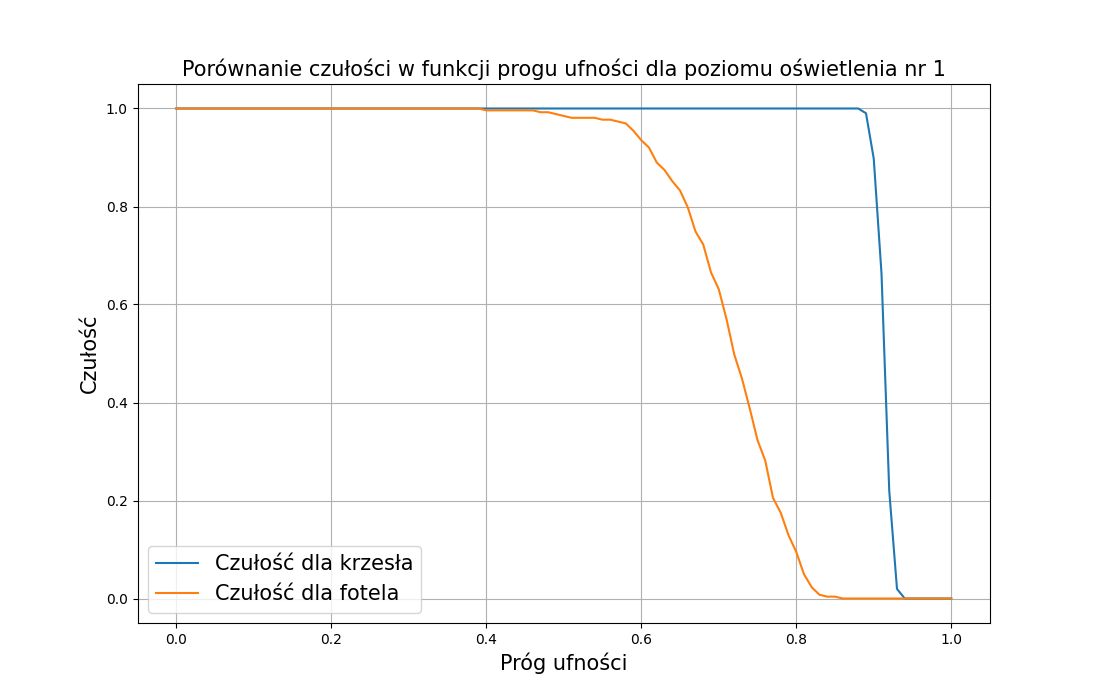
\includegraphics[width=\linewidth]{r_test_dokładności/chair_charts/1.png}
    \caption{Porównanie czułości w funkcji progu ufności dla krzesła i fotela. Poziom oświetlania nr 1.}
    \label{fig:chair-game-1}
\end{figure}

\begin{figure}[H]
    \centering
    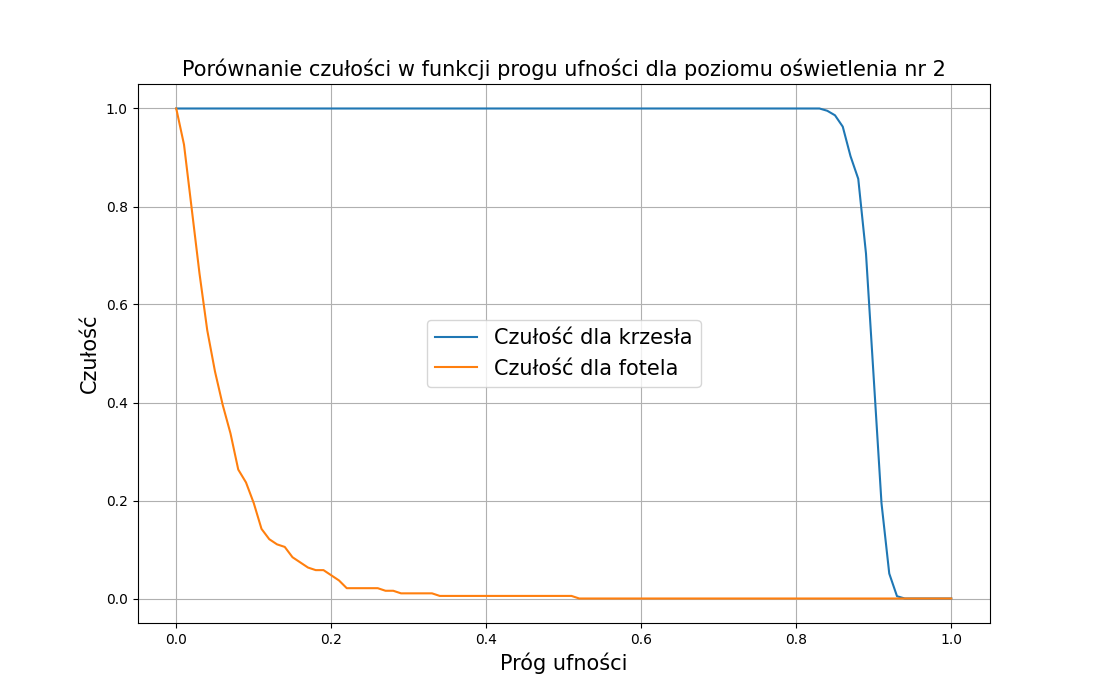
\includegraphics[width=\linewidth]{r_test_dokładności/chair_charts/2.png}
    \caption{Porównanie czułości w funkcji progu ufności dla krzesła i fotela. Poziom oświetlania nr 2.}
    \label{fig:chair-game-2}
\end{figure}

\begin{figure}[H]
    \centering
    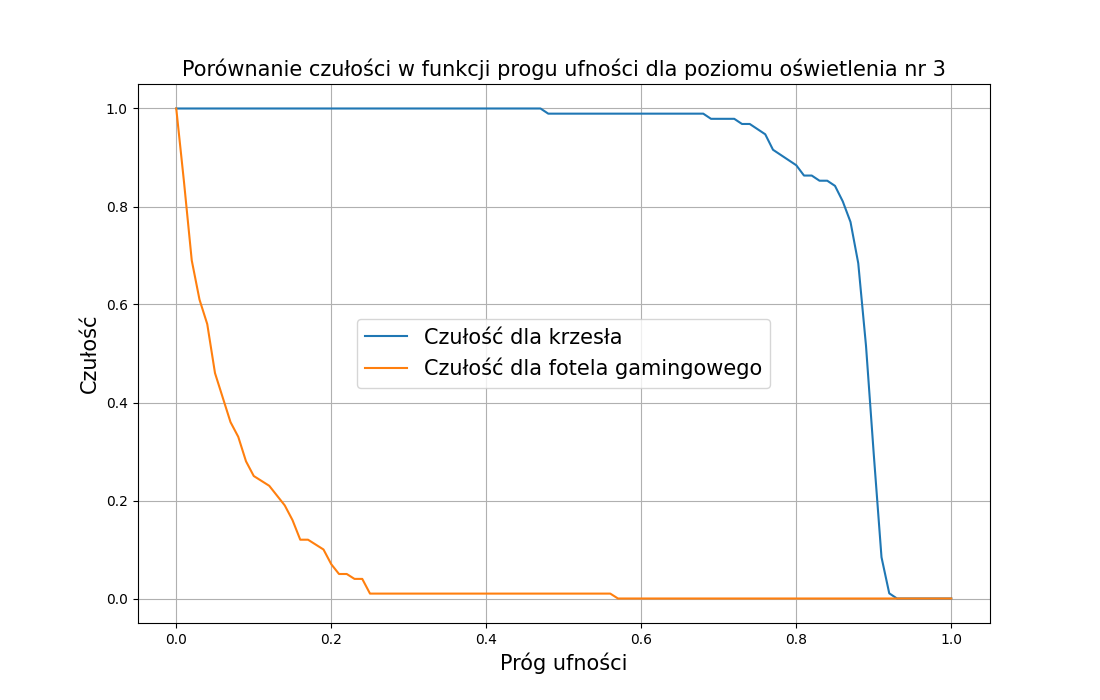
\includegraphics[width=\linewidth]{r_test_dokładności/chair_charts/3.png}
    \caption{Wykres do porównania czułości w funkcji progu ufności dla krzesła i fotela. Poziom oświetlania nr 3.}
    \label{fig:chair-game-3}
\end{figure}

\begin{figure}[H]
    \centering
    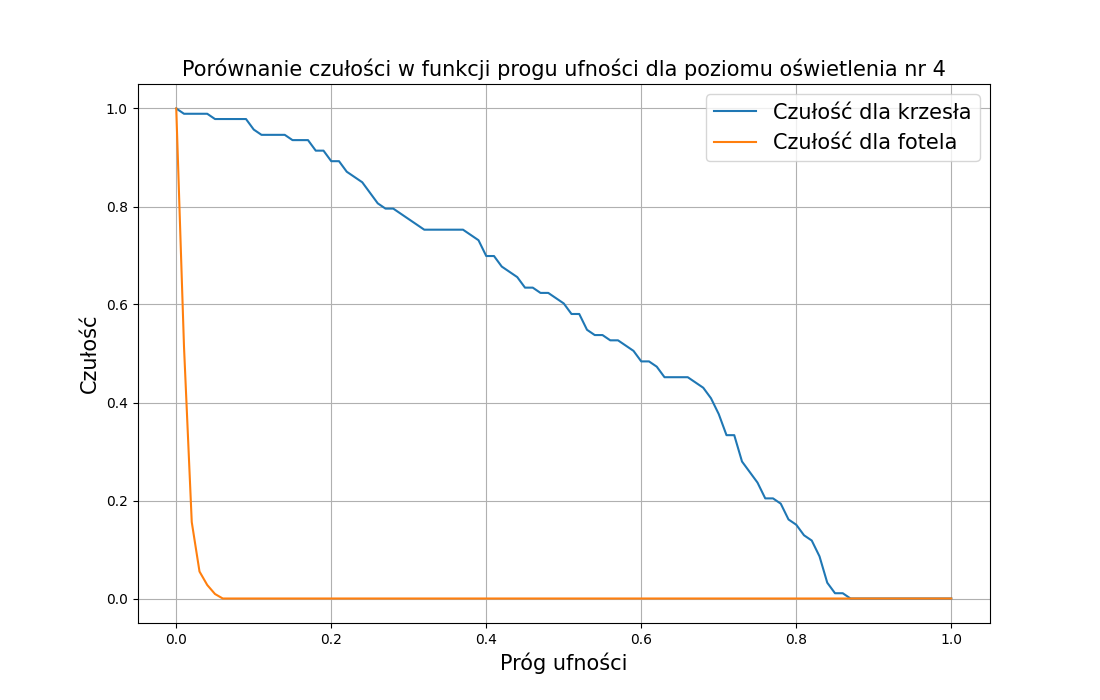
\includegraphics[width=\linewidth]{r_test_dokładności/chair_charts/4.png}
    \caption{Wykres do porównania czułości w funkcji progu ufności dla krzesła i fotela. Poziom oświetlania nr 4.}
    \label{fig:chair-game-4}
\end{figure}

\begin{figure}[H]
    \centering
    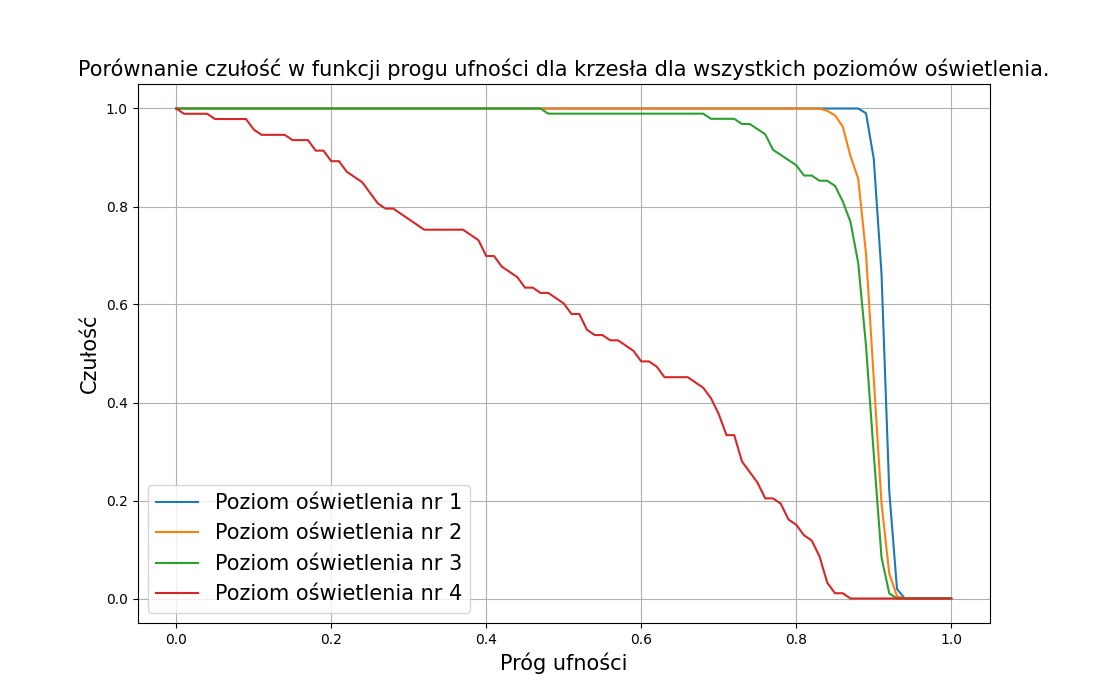
\includegraphics[width=\linewidth]{r_test_dokładności/chair_charts/chair.png}
    \caption{Wykres do porównania czułości w funkcji progu ufności dla wszystkich poziomów oświetlania. Obiekt --  krzesło.}
    \label{fig:all_bright_chair}
\end{figure}

\begin{figure}[H]
    \centering
    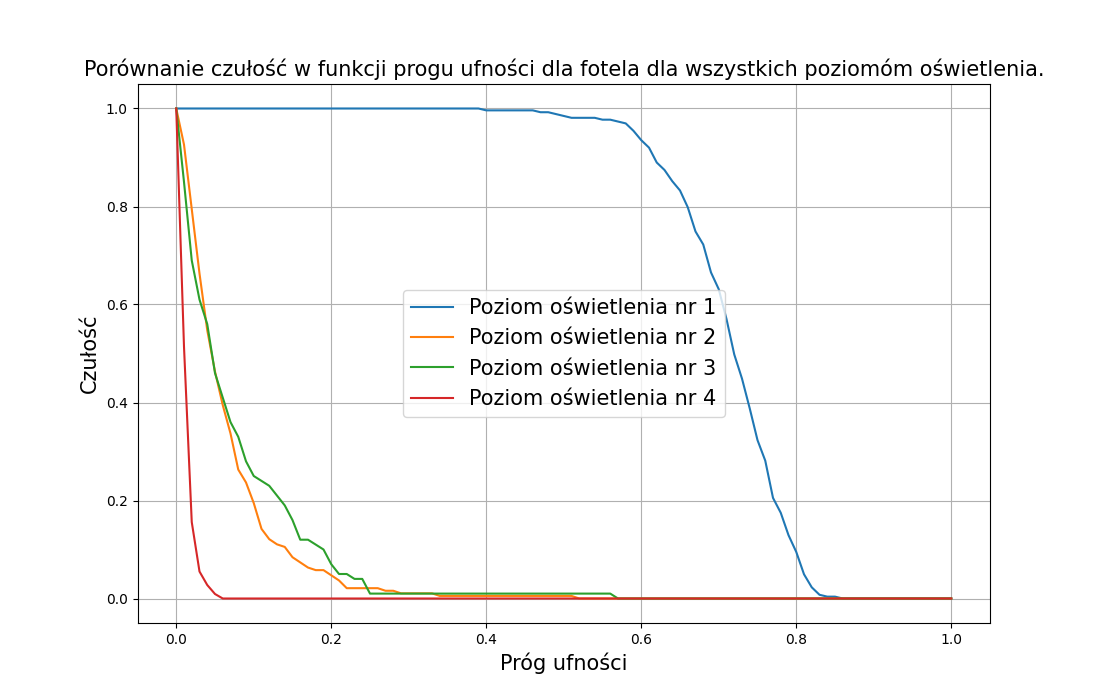
\includegraphics[width=\linewidth]{r_test_dokładności/chair_charts/gaming-chair.png}
    \caption{Wykres do porównania czułości w funkcji progu ufności dla wszystkich poziomów oświetlania. Obiekt --  fotel.}
    \label{fig:all_bright_game}
\end{figure}